\subsection{Recycle results}

\begin{frame}
    \frametitle{Recycling scheme dictates amount of separated material}
    \begin{itemize}
        \item Scenario 16 (Continuous reprocessing) has the 
              most separated material 
        \item Scenario 15 (Limited, no TRISO) has the least separated 
              material
    \end{itemize}
    \begin{figure}
        \centering
        \begin{subfigure}{0.495\textwidth}
            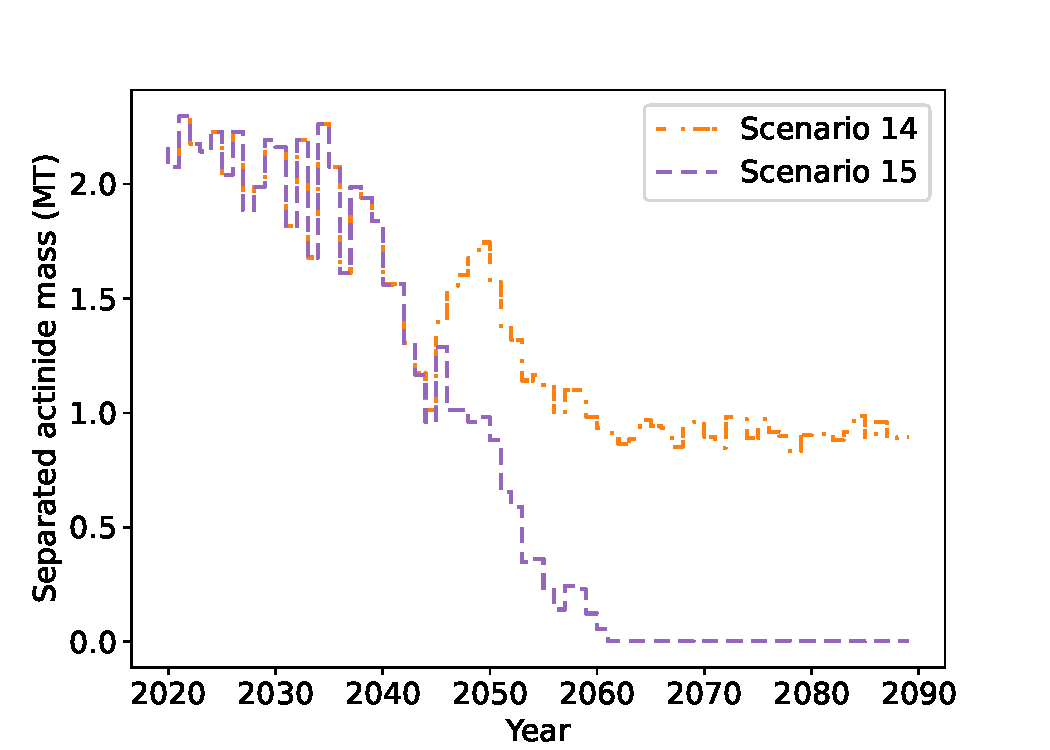
\includegraphics[width=1.1\linewidth]{nogrowth_recycle_sep_pu_limited.pdf}
            \caption{Annual average mass in Scenarios 14-15}
        \end{subfigure}
        \hfill
        \begin{subfigure}{0.495\textwidth}
            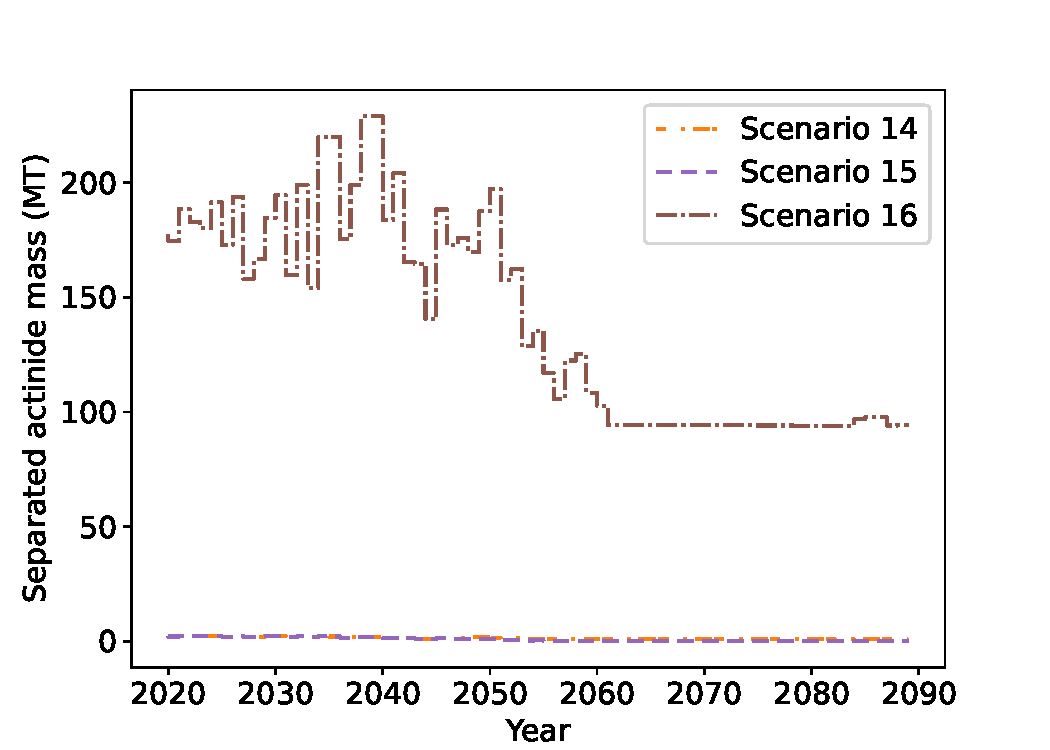
\includegraphics[width=1.1\linewidth]{nogrowth_recycle_sep_pu.pdf}
            \caption{Annual average mass in Scenarios 14-16}
        \end{subfigure}
        \caption{Separated actinide masses for advanced reactors in Scenarios 14-16}
        \label{fig:recycle_sep_pu}
    \end{figure}
\end{frame}

\begin{frame}
    \frametitle{Recycling decreases HALEU needs}
    \begin{itemize}
        \item Scenario 15 (Limited, no TRISO) requires the most 
              enriched uranium, has least plutonium-based fuel
        \item Scenario 16 (Continuous reprocessing) doesn't 
              require any enriched uranium, most plutonium-based fuel
    \end{itemize}
    \begin{figure}
        \centering
        \begin{subfigure}{0.495\textwidth}
            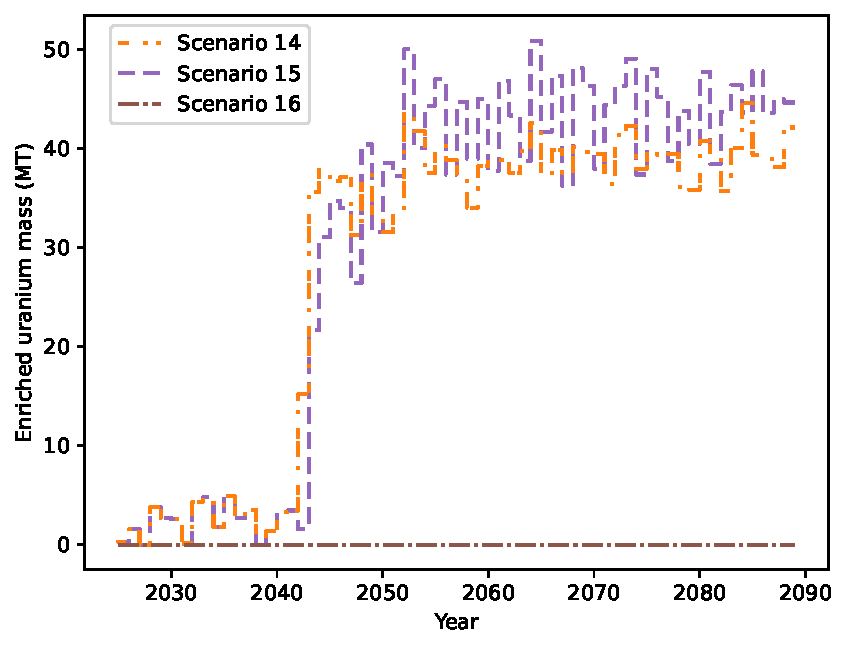
\includegraphics[width=1.01\linewidth]{nogrowth_recycle_Uaverages.pdf}
            \caption{Uranium-based fuel mass}
        \end{subfigure}
        \hfill
        \begin{subfigure}{0.495\textwidth}
            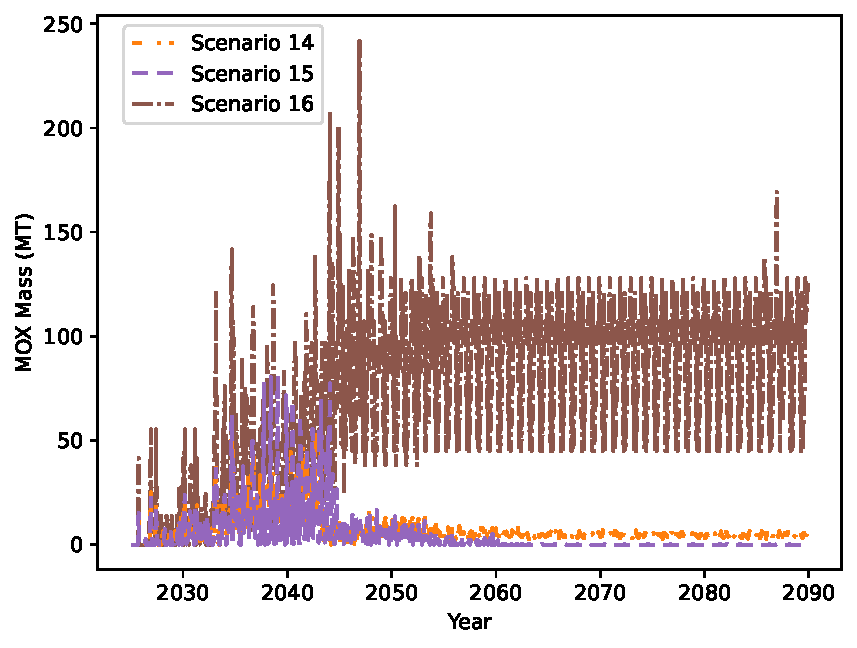
\includegraphics[width=1.01\linewidth]{nogrowth_recycle_MOX.pdf}
            \caption{Plutonium-based fuel mass}
        \end{subfigure}
        \caption{Fuel masses for advanced reactors in Scenarios 14-16}
        \label{fig:recycle_fuel}
    \end{figure}
\end{frame}

\begin{frame}
    \frametitle{Transition analysis conclusions}
    \begin{itemize}
        \item The advanced reactors deployed drive the materials required 
              for each scenario
        \item Reprocessing decreases \gls{HALEU} needs 
        \item Decrease in \gls{HALEU} needs is driven by the material 
              available for reprocessing and the material separated 
              from \gls{UNF}
        \item<2-> These scenarios consider large changes in the transition. 
             What about small changes?
    \end{itemize}
\end{frame}